\section*{Question 1}
\emph{Investigate the stability and accuracy of the four schemes in terms of the Courant-Friedrichs-Lewy (CFL) numbers $\lambda = c \tfrac{dt}{dx}$ and $\mu = \nu \tfrac{dt}{{dx}^2}$. In particular use numerical experimentation and/or von Neumann stability analysis to determine stability boundaries.}

\lstinputlisting[label=code1, language=Octave, caption=Code used to find the maximum time step and the resulting CFL parameters]{probe2.m}

The stability boundary is probed numerically through the script in Listing \ref{code1} by iterating the provided \texttt{wave.m}, which was changed to accept values of $c$ and $\nu$ and return a boolean flag to whether the function is stable or not. Since the energy is supposed to decay with each iteration due to losses from viscosity, a final energy value higher than the initial should indicate that the problem has become unstable. The ranges of $c$ and $\nu$ are created using a \texttt{linspace} command and starting from values close to $0$ to avoid instabilities especially for Euler based evolutions. Figures \ref{euler} and \ref{rk2} show the stability for the four combinations of space and time differencing formulas.

\begin{figure}[ht!]
\centering
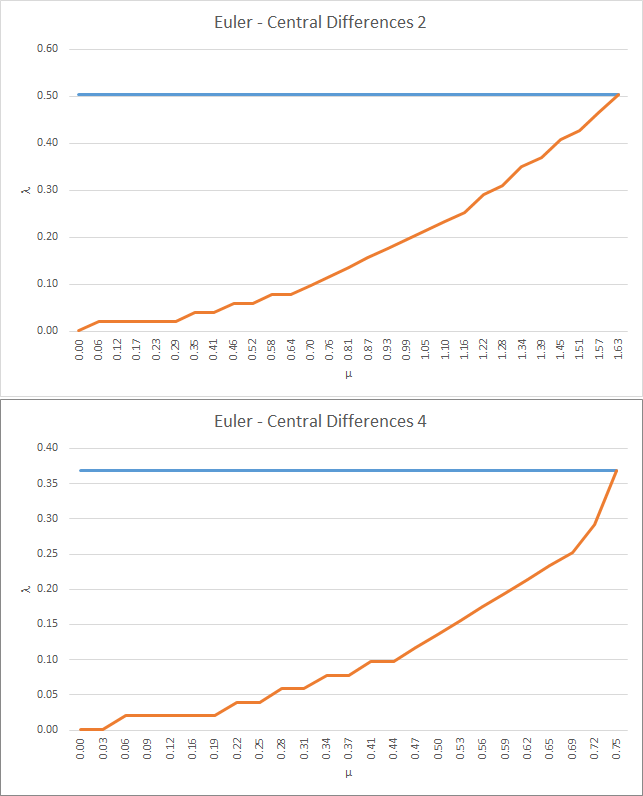
\includegraphics[scale=0.8]{./TEXT/Euler.png}
\caption{Euler time stepping with $2^{nd}$ and $4^{th}$ order Central Differences}
\label{euler}
\end{figure}

The main differences between using \nth{2} and \nth{4} Central Differences is that the upper stability boundary is lowered from $\lambda \approx 0.5$ in the CD2 case to $\lambda \approx 0.37$ in the CD4 case. The lower value for CD4 is expected due to the fact that more nearby spatial mesh points are required to propagate the solution to the next time step accurately. The lower stability boundary (in orange) for Euler time-stepping is more linear than for Runge-Kutta 2 due to the fact that in RK2 the time step is 'divided' into a predicted value and a corrected one which can be compared to taking a smaller step size.

\begin{figure}[ht!]
\centering
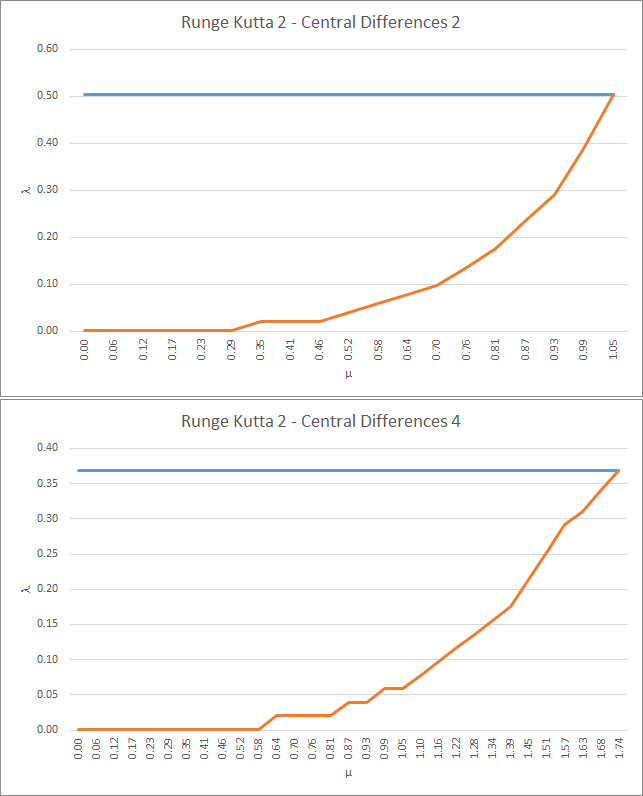
\includegraphics[scale=0.8]{./TEXT/RK2.png}
\caption{Runge-Kutta 2 time stepping with $2^{nd}$ and $4^{th}$ order Central Differences}
\label{rk2}
\end{figure}

The coarseness of the two ranges means that the exact moment when the instabilities start to grow are not captured, so the displayed graphs should be taken as an indication of general behaviour of the methods and not precise quantitative truth. It should also be noted that in some of the methods the values of $\mu$ become larger than $1$, which even though it is not displayed at that moment as an energy increase, it is an instability due to the fact that the lower frequencies are separated from the main wave and move slower. This behaviour is not captured by the comparison charts in the figures below and they should be seen, again, as an indication of general behaviour and not quantitative accuracy.
